\chapter[Introducción a los Tensores Cartesianos]{Introducción a los\breaktitle Tensores Cartesianos}

% Llegando al último capítulo del curso, nos desviamos un poco de la noción de que este curso se dedica a enseñar métodos matemáticos que pueden ser útiles en Física, para en su lugar introducir cantidades y conceptos con la misma utilidad.

Una de las nociones más importantes que tenemos en física clásica es el hecho de que \emph{los fenómenos físicos son los mismos, y no deben cambiar según el observador}, más allá de que las componentes de las cantidades que los describen puedan hacerlo. Particularmente, nos centraremos en las \emph{transformaciones ortogonales} de un sistema coordenado, referidas de forma más común como \textbf{rotaciones}. 

Por ejemplo, un vector que describe la posición de un objeto en función del tiempo puede ser diferente según el sistema de coordenadas en que se lo describa, pero el movimiento \emph{físico} del objeto seguirá siendo el mismo.

% \section{Sistemas Coordenados}

% Antes de entrar más de lleno en la discusión, recordemos e introduzcamos algunas definiciones.

% \begin{defi} \marginnote{Delta de Kronecker}
%     Se denomina \textbf{delta de Kronecker} al elemento $\delta_{ij}$, definido en un espacio vectorial de $n$ dimensiones como
%     \begin{equation}
%         \delta_{ij} = \begin{dcases}
%             1, \qquad i = j \\
%             0, \qquad i \neq j
%         \end{dcases} \ .
%     \end{equation} 

%     Este elemento puede representarse de forma matricial como la matriz identidad del espacio de dimensión $n$.
% \end{defi}

% \newpage

% \begin{defi} \marginnote{Base ortonormal}
%     Sea un conjunto de vectores unitarios $\left\{ \hat{e}_i\right\}_{i=1}^n$ de un espacio $n$-dimensional. Diremos que este forma una \textbf{base ortonormal} si al realizar el producto escalar entre elementos del conjunto, se cumple la relación
%     \begin{equation}
%         \hat{e}_i\cdot \hat{e}_j = \delta_{ij} \ ,
%     \end{equation}
%     donde $\delta_{ij}$ es la delta de Kronecker.
% \end{defi}

% \begin{defi} \marginnote{Vector posición}
%     Dado un sistema coordenado en un espacio de $n$ dimensiones, podemos definir el \textbf{vector posición} $\vec{x}$, que une el origen del sistema con punto con coordenadas $x_i$, con $i = 1, 2, \dots, n$ como
% \begin{equation} \label{eq:vector-posicion}
%     \vec{x} = \sum_{i=1}^n x_i \hat{e}_i \ ,
% \end{equation}
% donde las \textbf{componentes del vector} en la base $\{ \hat{e}_i\}_{i=1}^n$ pueden expresarse como
% \begin{equation}
%     x_i = \vec{x} \cdot \hat{e}_i \ .
% \end{equation}
% \end{defi}

% Más allá de que el vector posición es aquel que tiene un sentido \emph{físico} a partir del cual hacer las definiciones, podemos descomponer \emph{cualquier vector} en la base $\{ \hat{e}_i\}_{i=1}^n$ en términos de sus respectivas componentes, sin importar la cantidad que este pueda representar.


\section{Transformaciones Ortogonales}

Cuando estamos trabajando con coordenadas cartesianas, podemos definir un nuevo sistema coordenado, que llamaremos $x'_i$ y cuya base es $\{ \hat{e}_i'\}_{i=1}^n$, que corresponde a una \emph{rotación} del sistema $x_i$ definido anteriormente, como se ve en la figura \ref{fig:bases-ortonormales}.

\begin{figure}[htbp]
    \centering
    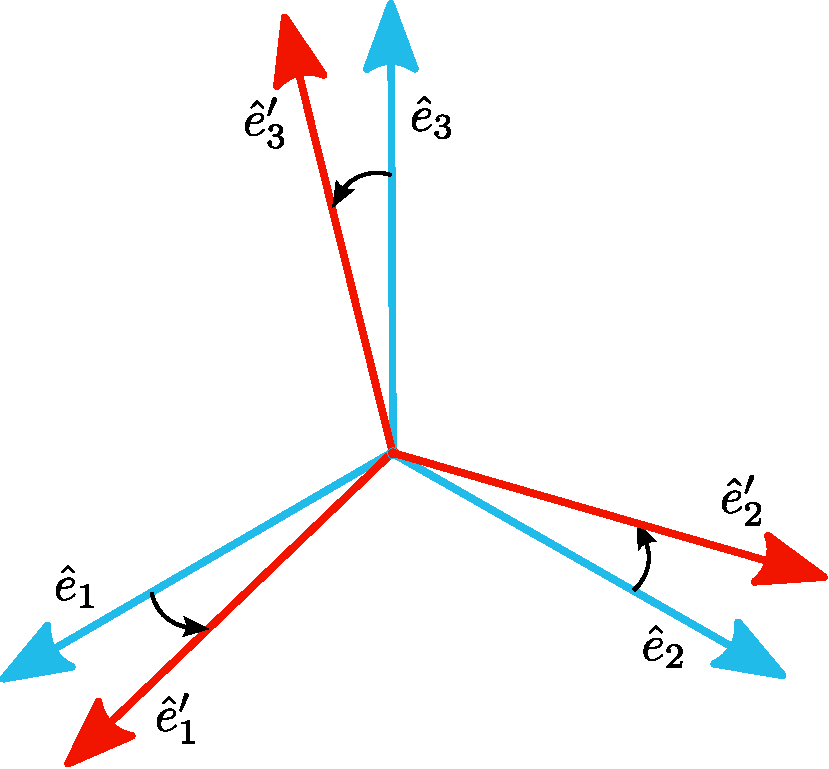
\includegraphics[width=6cm]{Figuras/fig-rotacion-bases.pdf}
    \caption{Una transformación ortogonal de dos bases ortonotmales en 3 dimensiones, $\hat{e}_i$ y $\hat{e}'_j$}
    \label{fig:bases-ortonormales}
\end{figure}

Respecto de esta nueva base, un vector $\vec{v}$ cualquiera puede ser descompuesto en sus componentes $v_i'$ \emph{en la base} $\{ \hat{e}_i'\}_{i=1}^n$,
\begin{equation}
    \vec{v} = \sum_{i=1}^n v_i' \hat{e}'_i \ .
\end{equation}

Dado que, si bien dan origen a sistemas de coordenadas diferentes, ambas bases se encuentran en el mismo espacio vectorial, ¿Cómo podemos relacionar ambas bases entre sí? Para ello, haremos uso de una \textbf{matriz de transformación}, definida como
\begin{equation}
    A = \begin{pmatrix}
        a_{11} & a_{12} & \dots & a_{1n} \\
        a_{21} & a_{22} & \dots & a_{2n} \\
        \vdots & \vdots & \ddots & \vdots \\
        a_{n1} & a_{n2} & \dots & a_{nn}
    \end{pmatrix} =
    \begin{pmatrix}
        \hat{e}_1 \cdot \hat{e}'_1 & \hat{e}_1 \cdot \hat{e}'_2 & \dots & \hat{e}_1 \cdot \hat{e}'_n \\
        \hat{e}_2 \cdot \hat{e}'_1 & \hat{e}_2 \cdot \hat{e}'_2 & \dots & \hat{e}_2 \cdot \hat{e}'_n \\
        \vdots & \vdots & \ddots & \vdots \\
        \hat{e}_n \cdot \hat{e}'_1 & \hat{e}_n \cdot \hat{e}'_2 & \dots & \hat{e}_n \cdot \hat{e}'_n
    \end{pmatrix} \ .
\end{equation}

De este modo, un vector de la base $\vec{e}'_i$ puede escribirse también en términos de la base $\vec{e}_i$,
\begin{equation} \label{eq:transformacion-coordenadas}
    \hat{e}'_i = \sum_{j=1}^n a_{ij} \hat{e}_j \ ,
\end{equation}
por lo que podemos reescribir el vector $\vec{v}$ como
\begin{equation} \label{eq:transformacion-vector}
    \vec{v} = \sum_{i=1}^n v'_i \left( \sum_{j=1}^n a_{ij} \hat{e}_j \right) \ .
\end{equation}

\subsection{Convenio de suma de Einstein}

Antes de continuar la discusión, es útil introducir el  \textbf{convenio de suma de Einstein}, que establece que en toda expresión donde se repitan dos índices iguales, \emph{existe una suma implícita sobre todo el rango de variación del índice}. Es más, el índice de suma \emph{es una etiqueta arbitraria}, por lo que puede ser renombrada a conveniencia.

Por ejemplo, las expresiones \eqref{eq:vector-posicion} y \eqref{eq:transformacion-vector} pueden reescribirse como
\begin{align}
    \vec{v} & = v_i \hat{e}_i \, , \\
    \vec{v} & = v'_i a_{ij} \hat{e}_j .
\end{align}

Además, dado que existe una suma implícita, podemos aplicar la delta de Kronecker para reemplazar índices en una multiplicación, de modo que
\begin{equation}
    a_{ij} b_{jk} \delta_{ki} = a_{ij} b_{ji} = a_{kj} b_{jk} \ .
\end{equation}


La discusión hecha hasta ahora es válida para cualquier transformación de coordenadas entre dos bases distintas. Para los efectos de este curso, nos interesa trabajar únicamente con \emph{transformaciones ortogonales}.

\begin{defi} \marginnote{Transformación ortogonal}
    Una \textbf{transformación ortogonal} es aquella transformación de cambio de base que permite convertir una base ortonormal $\{\hat{e}_i\}_{i=1}^n$ en una nueva base ortonormal $\{\hat{e}'_i\}_{i=1}^n$.
\end{defi}

Para asegurarnos que la transformación \eqref{eq:transformacion-coordenadas} sea una transformación ortogonal, debe además satisfacer que
\begin{align}
    \delta_{ij} & = \hat{e}'_i \cdot \hat{e}'_j \\
    & = \left( \sum_{k=1}^n a_{ik} \hat{e}_k \right) \left( \sum_{l=1}^n a_{jl} \hat{e}_l \right) \\
    & = \sum_{k=1}^n \sum_{l=1}^n a_{ik} a_{jl} (\hat{e}_k \cdot \hat{e}_l) \\
    & = \sum_{k=1}^n \sum_{l=1}^n a_{ik} a_{jl} \delta_{kl} \\
    & = \sum_{k=1}^n a_{ik} a_{jk} \ , \label{eq:delta-transformacion-ortogonal}
\end{align}
o bien, matricialmente,
\begin{equation}\label{eq:condicion-matricial}
    A \cdot (A^T) = I \ ,
\end{equation}
que al calcular el determinante, observamos que
\begin{equation}
    \det(A)^2 = 1 \ , 
\end{equation}
de modo que una transformación ortogonal deberá satisfacer que $\det(A) = 1$, caso en que se denomina \emph{transformación propia}, o bien que $\det(A) = -1$, lo que se conoce como \emph{transformación impropia}.

En particular, de \eqref{eq:condicion-matricial} podemos observar que para una transformación ortogonal, $A^T = A^{-1}$, es decir, la transpuesta de la transformación coincide con su inversa, de modo que también se satisface que
\begin{equation}
    (A^T) \cdot A = I \ ,
\end{equation}
o en notación indicial,
\begin{equation}
    \sum_{k=1}^n a_{ki} a_{kj} =  \delta_{ij} \ .
\end{equation}

\section{Tensores Cartesianos}

Hasta ahora, hemos discutido las propiedades de los vectores, elementos con los que ya somos familiares. Sin embargo, seguimos sin responder la incógnita de \emph{¿qué es un tensor?}. Para ello, introduzcamos una operación entre vectores.

\begin{defi}\marginnote{Producto externo}
    Dados dos vectores $\vec{u} = u_i \hat{e}_i$ y $\vec{v} = v_i \hat{e}_i$, se define el \textbf{producto externo} entre ambos vectores como la cantidad
    \begin{equation}
        T_{ij} = u_i v_j \ .
    \end{equation}
\end{defi}

Como podemos ver de la definición anterior, necesitamos de \emph{dos índices} para definir el producto externo. ¿Qué ocurre con esta cantidad si, en lugar de utilizar la base $\hat{e}_i$, utilizamos la base $\hat{e}'_i$? En otras palabras, ¿cómo transforma $T_{ij}$ bajo transformaciones ortogonales? Notamos que
\begin{equation}
    T'_{ij} = u'_i v'_j = (a_{ik}u_k)(a_{jl} v_l) = a_{ik} a_{jl} (u_k v_l) =  a_{ik} a_{jl} T_{kl} \ .
\end{equation}

Observamos pues, que $T_{ij}$ transforma de manera similar a los vectores bajo transformaciones ortogonales. A cantidades que siguen una regla de transformación de este tipo, las llamamos \emph{tensores (cartesianos) de rango 2}, pues requerimos de dos matrices de transformación para definirlas adecuadamente. Observamos que, para un espacio de $n$ dimensiones, estos elementos tendrán $n^2$ componentes.

Esta noción puede ampliarse a más dimensiones, según la siguiente definición,
\begin{defi} \marginnote{Tensor cartesiano}
    Dado un espacio de $n$ dimensiones, el conjunto de $n^r$ cantidades $T_{i_1 i_2 \dots i_r}$ definidas en cada sistema ortogonal de coordenadas, son las componentes de un \textbf{tensor cartesiano de rango} $\mathbf{r}$ si, bajo transformaciones ortogonales, sus valores siguien la regla de transformación
    \begin{equation}
        T'_{i_1 i_2 \dots, i_r} = a_{i_1 j_1} a_{i_2 j_2} \dots a_{i_r j_r} T_{j_1 j_2 \dots j_r} \ . 
    \end{equation}
\end{defi}

Gracias a esta definición, observamos que los \textbf{vectores}, que tienen una sola matriz de transformación en su definición \eqref{eq:transformacion-vector}, son \emph{tensores de rango 1}. A su vez, los \textbf{escalares} son cantidades que no se ven modificadas frente a una transformación de coordendas, de modo que $\rho' = \rho$. Por ello, podemos considerarlos \emph{tensores de rango 0}.

\begin{ejemplo}
    \textbf{Tensor de inercia.}

    Consideremos un cuerpo con densidad $\rho(x_i)$, contenido en una región $V$ que rota \emph{rígidamente} respecto de un eje con dirección $\hat{\omega}$ con velocidad angular $\omega$. Entonces, podemos hallar su momento angular respecto al origen del sistema (ubicado sobre el eje de rotación) como
    \begin{align*}
        \vec{L} & = \int_V \x \times d\vec{p} \\
        & = \int_V \rho(x) \x \times \vec{v} \ dV \\
        & = \int_V \rho(x) \x \times (\vec{\omega} \times \x) \ dV \ .
    \end{align*}
    Usando la identidad $\vec{A} \times (\vec{B} \times \vec{C}) = \vec{B} (\vec{A} \cdot \vec{C}) - \vec{C} (\vec{A} \cdot \vec{B})$, podemos escribir
    \begin{equation*}
        \vec{L} = \int_V \rho(x) [\vec{\omega}(\x \cdot \x) - \x (\vec{\omega} \cdot \x)] \ dV \ ,
    \end{equation*}
    o en términos de las componentes del vector,
    \begin{align*}
        L_i & = \int_V \rho(x) [\omega_i(x_k x_k) - x_i(\omega_j x_j)] \ dV \\
        & = \int_V \rho(x) [(\delta_{ij} \omega_j)(x_k x_k) - x_i(\omega_j x_j)] \ dV \\
        & = \left( \int_V \rho(x) [\delta_{ij} (x_k x_k) - x_i x_j] \ dV \right) \omega_j \ ,
    \end{align*}
    es decir, 
    \begin{equation*}
        L_i = I_{ij} \omega_j \, 
    \end{equation*}
    donde $I_{ij}$ es el \emph{tensor de inercia} definido como
    \begin{equation*}
        \int_V \rho(x) [\delta_{ij} (x_k x_k) - x_i x_j] \ dV \ .
    \end{equation*}

    ¿Es esta cantidad efectivamente un tensor cartesiano? Revisemos cómo transforma bajo una transformación ortogonal,
    \begin{align*}
        I'_{ij} & = \int_V \rho'(x') [\delta_{ij} (x'_k x'_k) - x'_i x'_j] \ dV' \\
        & = \int_V \underbrace{\rho(x)}_{\text{Escalar}} [\delta_{ij}\underbrace{(x_k x_k)}_\text{Escalar} - (a_{il} x_l)(a_{jm} x_m)] \ dV \\
        & = \int_V \rho(x) [(a_{il}a_{jl})(x_k x_k) - (a_{il} x_l)(a_{jm} x_m)] \ dV \\
        & = \int_V \rho(x) [(a_{il}a_{jm}\delta_{lm})(x_k x_k) - (a_{il} x_l)(a_{jm} x_m)] \ dV \\
        & = (a_{il} a_{jm}) \int_V \rho(x) [(\delta_{lm})(x_k x_k) - x_l x_m] \ dV \\
        & = a_{il} a_{jm} I_{lm} \ ,
    \end{align*}
    de modo que efectivamente $I_{jl}$ transforma como un tensor cartesiano.
\end{ejemplo}

\subsection{Propiedades}

En este contexto, vale la pena mencionar con algo más de detalle a dos propiedades.

\begin{propiedad}
    \textbf{Propiedades de los tensores cartesianos.}

    \begin{enumerate}
        \item Si \emph{todas las componentes de un tensor se anulan en un sistema coordenado ortogonal}, ellas se anularán \emph{en todo sistema coordenado ortogonal}.  Esta propiedad nos interesa, ya que nos indica que la anulación de un tensor \textbf{es una propiedad intrínseca} de este. De esta propiedad surge la importancia de utilizar tensores en Física, pues nos permite plantear leyes \emph{que no dependen del sistema coordenado en que trabajamos}, sino únicamente del fenómeno estudiado.
        
        Por ejemplo, podemos estar estudiando el momento de inercia de un cuerpo en movimiento, el cual es un tensor de rango 2. Si diera la casualidad de que este es cero en algún sistema coordenado ortogonal, esto quiere decir que, \textbf{en cualquier sistema coordenado ortogonal}, el cuerpo \emph{no se encuentra rotando}.
    
        \item Existen algunos \textbf{tensores invariantes} o \textbf{isotrópicos}, los cuales tienen siempre las mismas componentes \emph{en cualquier sistema coordenado}. Un ejemplo de estos es la delta de Kronecker, pues en cualquier sistema coordenado tendrá las mismas componentes, 1 si $i=j$ y 0 si $i\neq j$.
        
        En efecto, podemos observar que la delta de Kronecker transforma como
        \begin{equation}
            \delta'_{ij} = a_{ik} a_{jl} \delta_{kl} = a_{ik} a_{jk} = \delta_{ij} \ .
        \end{equation}
    \end{enumerate}
\end{propiedad}



\section{Álgebra Tensorial}

Dicho rápido y sencillo, hemos visto que los tensores de rango 1 y rango 2 se comportan como vectores columna y como matrices, respectivamente. Por ello, esperaríamos que sea posible definir operaciones tensoriales similares a las definidas para estos elementos, incluyendo la posibilidad de construir tensores a partir de otros.

\begin{itemize}
    \item \textbf{Adición y sustracción.} Se define la adición (o suma) y sustracción (o resta) de dos tensores \emph{del mismo orden} componente a componente, es decir,
    \begin{align}
        S_{ij \dots k} & = V_{ij \dots k} + W_{ij \dots k} \ , \\
        D_{ij \dots k} & = V_{ij \dots k} - W_{ij \dots k} \ .
    \end{align}
    % \item \textbf{Producto por escalar.}
    \item \textbf{Permutación de índices.} La operación de permutar dos índices de un tensor de rango $r$, define un nuevo tensor de rango $r$. Es decir, dado un tensor $T_{ijk \dots l}$ de rango $r$, la cantidad
    \begin{equation}
        B_{ijk \dots l} = T_{ikj \dots l} 
    \end{equation}
    es también un tensor de rango $r$.

    \item \textbf{Producto tensorial, o directo.} De manera similar al \emph{producto externo} de dos vectores que calculamos anteriormente, podemos definir el producto entre dos tensores de diferente rango, digamos $r$ y $s$, lo que permite formar un nuevo vector de rango $r+s$,
    \begin{equation}
        C_{i_1 i_2 \dots i_{r+s}} = A_{i_1 i_2 \dots i_r} \cdot B_{i_{r+1} i_{r+2} \dots i_{r+s}} \ .
    \end{equation}
    
    En este caso, es relevante respetar la posición de los índices en el producto, pues en general el tensor $C_{ij} = A_i B_j$ será distinto al vector $D_{ij} = A_j B_i$, como consecuencia de la permutación de índices.

    Esta operación incluye, por supuesto, el producto entre un tensor de rango 0 (un escalar) y un tensor de rango $r$, definiendo el \emph{prodcuto por un escalar}.

    \item \textbf{Contracción de índices.} El producto escalar entre dos vectores nos entrega un escalar en lugar de un tensor de orden 2, como consecuencia de la repetición de índices en el producto. De manera similar, la repetición de dos índices dentro de un tensor de orden $r$ (digamos, el $s$-ésimo y el $t$-ésimo índice), es equivalente a un tensor de orden $r-2$,
    \begin{equation}
        B_{i_1 i_2 \dots i_{r-2}} = A_{i_1 i_2 \dots j \dots j \dots i_{r-2}} \ ,
    \end{equation}
    o de forma equivalente,
    \begin{equation}
        B_{i_1 i_2 \dots} = A_{i_1 i_2 \dots i_r} \delta_{i_s i_t} \ .
    \end{equation}

    \item \textbf{Ley del cociente.} Consideremos el caso en que tenemos una expresión de la forma
    \begin{equation}\label{eq:ley-cociente}
        A_{pq \dots k \dots m} B_{ij \dots k \dots n} = C_{pq \dots m ij \dots n} \ ,
    \end{equation}
    donde sabemos que $B$ y $C$ son tensores de rango $r$ y $s$, respectivamente, pero desconocemos si $A$ es un tensor. La ley del cociente establece que \emph{si la relación \eqref{eq:ley-cociente} es válida en cualquier sistema de coordenadas, entonces} $A$ es un tensor de orden $s-r+2$. La demostración (para el caso $r=s=2$) puede ser hallada en el capítulo 26, sección 7 de Riley \cite{Riley}.
    
    \item \textbf{Simetría.} Cuando un tensor no cambia bajo la permutación de dos de sus índices, 
    \begin{equation}
        T_{i_1 i_2 \dots i_s \dots i_t \dots i_r} = T_{i_1 i_2 \dots i_t \dots i_s \dots i_r} \ , 
    \end{equation}
    se dice que este es \emph{simétrico} respecto a dichos índices. Si, en cambio,
    \begin{equation}
        T_{i_1 i_2 \dots i_s \dots i_t \dots i_r} = - T_{i_1 i_2 \dots i_t \dots i_s \dots i_r} \ ,
    \end{equation}
    decimos que el tensor es \emph{antisimétrico} respecto de dichos índices. En general, un tensor de rango $r$ puede escribirse como la suma de un tensor simétrico y un tensor antisimétrico respecto de la misma permutación de índices, de modo que
    \begin{align}
        T_{i_1 i_2 \dots i_s \dots i_t \dots i_r} & = \frac{1}{2} (T_{i_1 i_2 \dots i_s \dots i_t \dots i_r} + T_{i_1 i_2 \dots i_t \dots i_s \dots i_r}) + \frac{1}{2}(T_{i_1 i_2 \dots i_s \dots i_t \dots i_r} - T_{i_1 i_2 \dots i_t \dots i_s \dots i_r}) \\
        & = S_{i_1 i_2 \dots i_s \dots i_t \dots i_r} + A_{i_1 i_2 \dots i_s \dots i_t \dots i_r} \ .
    \end{align}

    En física, a veces es común utilizar la siguiente notación,
    \begin{align}
        T_{i_1 i_2 \dots (i_s| \dots |i_t) \dots i_r} & \equiv S_{i_1 i_2 \dots i_s \dots i_t \dots i_r} \ , \\
        T_{i_1 i_2 \dots [i_s| \dots |i_t] \dots i_r} & \equiv A_{i_1 i_2 \dots i_s \dots i_t \dots i_r} \ ,
    \end{align}
    donde los índices entre paréntesis o corchetes son los índices respecto de los cuales el tensor es simétrico o antisimétrico.

    Un tensor \textbf{completamente simétrico} de rango $r$ es aquel que es simétrico respecto a la permutación de cada par de índices. Este tendrá $\frac{(n+r-1)!}{(n-1)! r!}$ componentes linealmente independientes.

    De forma análoga, un tensor \textbf{completamente antisimétrico} de rango $r$ es aquel que es antisimétrico respecto a la permutación de cada par de índices. Este tendrá $\frac{n!}{(n-r)! r!}$ componentes linealmente independientes. En particular, un tensor de rango $r=n$, tendrá \emph{una única componente linealmente independiente}.
\end{itemize}


\section{Diagonalización de tensores de rango 2}

Una transformación ortogonal de especial interés es aquella que convierte a un tensor a una base en la que este es \emph{diagonal}, es decir, donde todos los elementos fuera de la diagonal principal son nulos, $T_{ij} = 0$, si $i \neq j$. En este caso, las componentes del tensor transforman de la siguiente forma:
\begin{equation}
    T'_{ij} = \sum_k \lambda_k \delta_{ik} \delta_{jk} \ ,
\end{equation}
donde $\lambda_k$ es una constante. En este caso, llamaremos a $\lambda_k$ un \textbf{valor propio}, o \textbf{autovalor} del tensor $\check{T} = T_{ij} \hat{e}_i \hat{e}_j$, asociado a un \textbf{vector propio} o \textbf{autovector} $\hat{e}'_k$, tal que se satisface la ecuación
\begin{equation}
    \check{T} \cdot \hat{e}'_k = \lambda_k \hat{e}'_k \ ,
\end{equation}
también escrita como 
\begin{equation}
    (T_{ij} - \lambda_k \delta_{ij}) \hat{e}_i (\hat{e}_j \cdot \hat{e}'_k) = (T_{ij} - \lambda_k \delta_{ij}) \hat{e}_i a_{jk} = 0
\end{equation}
o matricialmente,
\begin{equation} \label{eq:descomposicion}
    \begin{pmatrix}
        T_{11} - \lambda_k & T_{12} & \cdots \\
        T_{21} & T_{22} - \lambda_k & \cdots \\
        \vdots & \vdots & \ddots
    \end{pmatrix} 
    \begin{pmatrix}
        a_{ik} \\ a_{2k} \\ \vdots
    \end{pmatrix}
     = 
    \begin{pmatrix}
        0 \\ 0 \\ \vdots
    \end{pmatrix} \ .
\end{equation}

Para que la solución a esta ecuación sea no trivial, necesitamos que se satisfaga la \textbf{ecuación característica}
\begin{equation}
    \det(\check{T} - \lambda_k I) = 0 \ ,
\end{equation}
ecuación que corresponderá a un polinomio de grado $n$ el $\lambda_k$ si trabajamos en un espacio $n$-dimensional.

Reemplazando cada una de las raíces de este polinomio \emph{característico} en la ecuación \eqref{eq:descomposicion}, podemos hallar cada una de las componentes de la matriz de transformación $a_{jk}$, de modo que se satisfaga que la base ortonormal en que el tensor es diagonal se relacione con la base usual según la regla
\begin{equation}
    \hat{e}_k = a_{kj} \hat{e}_j \ .
\end{equation}

Llamaremos a la base diagonal como la \textbf{base de los ejes principales} del tensor, donde cada $\hat{e}'_k$ es uno de dichos ejes principales. Esta base es, por definición, ortogonal.

Una condición suficiente para que un tensor de rango 2 sea diagonalizable es que este sea \textbf{simétrico}.

\begin{ejemplo}
    \textbf{(Riley, sección 26.12)} La conductividad eléctrica en un cristal, $\check{sigma}$, es medida por un observador, quien determina que posee componentes
    \begin{equation*}
        [\sigma_{ij}] = \begin{pmatrix}
            1 & \sqrt{2} & 0 \\
            \sqrt{2} & 3 & 1 \\
            0 & 1 & 1
        \end{pmatrix} \ .
    \end{equation*}

    Si la densidad de corriente de un cristal viene dada por $\vec{J} = \check{\sigma} \vec{E}$, muestre que hay una dirección en el cristal a lo largo de la cual no puede fluir corriente. Además, determine si  la corriente puede fluir con la misma facilidad a lo largo de las otras dos direcciones perpendiculares.

    \textbf{Solución.} 

    La existencia de tres ejes principales para el cristal viene dada del hecho de que su conductividad es simétrica. De este modo, existe una base en la cual la conductividad es diagonal, y sus elementos no nulos corresponden a la conductividad en la dirección de cada uno de sus ejes principales. Entonces, podemos diagonalizarlo mediante el proceso antes descrito.

    Los autovalores pueden encontrarse a partir de la ecuación característica, de modo que 
    \begin{equation*} \left|
        \begin{array}{ccc}
            1 - \lambda & \sqrt{2} & 0 \\
            \sqrt{2} & 3 - \lambda & 1 \\
            0 & 1 & 1 - \lambda
        \end{array} \right| = 0 \ ,
    \end{equation*}
    a partir de la cual identificamos el polinomio característico
    \begin{equation*}
        (1-\lambda)[(3 - \lambda)(1-\lambda) - 1] - 2(1-\lambda) = (1-\lambda)[(3-\lambda)(1-\lambda) - 3] = (1-\lambda)(\lambda-4)\lambda = 0 \ ,
    \end{equation*}
    de modo que los autovalores de $\check{\sigma}$ asociados a sus ejes principales $\hat{e}'_1$, $\hat{e}'_2$ y $\hat{e}'_3$ son 4, 1 y 0, respectivamente. Entonces, podemos escribir
    \begin{equation*}
        [\sigma'_{ij}] = \begin{pmatrix}
            4 & 0 & 0 \\
            0 & 1 & 0 \\
            0 & 0 & 0 
        \end{pmatrix} \ ,
    \end{equation*}
    lo que, gracias a la ecuación $J_i' = \sigma'_{ij} E'_j$, muestra que en uno de los ejes principales (en el orden escogido, para $\hat{e}'_3$) no fluirá corriente, mientras que en los otros dos ejes principales, la corriente puede fluir con diferentes intensidades. 
\end{ejemplo}

También podría darse el caso de que nuestro proceso de diagonalización nos entregue autovalores \emph{degenerados}, es decir, asociados a más de un autovector. En estos casos, los autovectores no pueden determinarse de forma única, lo que implica que cualquier vector que se encuentre en el plano formado por los autovectores asociados a dicho autovalor es también un eje principal del tensor, asegurándonos siempre de que sean ortogonales entre sí.

\begin{ejemplo}
    Considere ahora un tensor de conductividad
    \begin{equation*}
        [\sigma_{ij}] = \begin{pmatrix}
            11 & -1 & 0 \\
            -1 & 11 & 0 \\
            0 & 0 & 10
        \end{pmatrix} \ .
    \end{equation*}
    Determine sus ejes principales.

    \textbf{Solución.}

    Dado que el tensor es simétrico, podemos asegurar la existencia de tres ejes principales perpendiculares entre sí.

    El polinomio característico de este tensor será dado por 
    \begin{equation*}
        (10 - \lambda)^2(\lambda - 12) = 0 \ ,
    \end{equation*}
    de modo que las raíces serán $\lambda_1 = 12$ y $\lambda_2 = \lambda_3 = 10$. Para la primera raíz, observamos que tenemos el sistema 
    \begin{equation*}
        \begin{pmatrix}
            -1 & -1 & 0 \\
            -1 & -1 & 0 \\
            0 & 0 & 2 \\
        \end{pmatrix}
        \begin{pmatrix}
            a_{11} \\ a_{12} \\ a_{13}
        \end{pmatrix}
        = \begin{pmatrix}
            0 \\ 0 \\ 0
        \end{pmatrix} \ .
    \end{equation*}

    Resolviendo el sistema, hallamos que 
    \begin{equation*}
        \begin{pmatrix}
            a_{11} \\ a_{12} \\ a_{13}
        \end{pmatrix}
        = \frac{1}{\sqrt{2}} \begin{pmatrix}
            1 \\ -1 \\ 0
        \end{pmatrix} \ ,
    \end{equation*}
    de modo que el primer eje principal, $\hat{e}'_1$, viene dado por
    \begin{equation*}
        \hat{e}'_1 = \frac{1}{\sqrt{2}}\hat{e}_1 - \frac{1}{\sqrt{2}}\hat{e}_2 \ .
    \end{equation*}

    Por otra parte, para los autovalores degenerados, tenemos los sistemas 
    \begin{equation*}
        \begin{pmatrix}
            1 & -1 & 0 \\
            -1 & 1 & 0 \\
            0 & 0 & 0 \\
        \end{pmatrix}
        \begin{pmatrix}
            a_{21} \\ a_{22} \\ a_{23}
        \end{pmatrix}
        = \begin{pmatrix}
            0 \\ 0 \\ 0
        \end{pmatrix} \ ,
    \end{equation*}
    y
    \begin{equation*}
        \begin{pmatrix}
            1 & -1 & 0 \\
            -1 & 1 & 0 \\
            0 & 0 & 0 \\
        \end{pmatrix}
        \begin{pmatrix}
            a_{31} \\ a_{32} \\ a_{33}
        \end{pmatrix}
        = \begin{pmatrix}
            0 \\ 0 \\ 0
        \end{pmatrix} \ ,
    \end{equation*}
    los que observamos que son idénticos.

    Resolviendo el sistema para $\lambda_2$, observamos que este nos impone la condición $a_{21} = a_{22}$, dejando libre el valor de $a_{23}$. Por conveniencia, podemos fijarlo a cero. Como este autovector debe ser ortonormal a $\hat{e}'_1$, tenemos que será de la forma
    \begin{equation*}
        \hat{e}'_2 = \frac{1}{\sqrt{2}} \hat{e}_1 + \frac{1}{\sqrt{2}} \hat{e}_2 \ .
    \end{equation*}

    Por último, $\hat{e}'_3$ también posee la condición $a_{31} = a_{32}$, con $a_{33}$ arbitrario. En este caso, para que sea ortonormal a $\hat{e}'_1$ y $\hat{e}'_2$, imponemos que $a_{31} = a_{32} = 0$, y que $a_{33} = 1$. De esta forma, $\hat{e}'_3 = \hat{e}_3$, y los ejes principales de este material serán 
    \begin{equation*}
        {\hat{e}'_1, \hat{e}'_2, \hat{e}'_3} = \left\{ \frac{1}{\sqrt{2}}(\hat{e}_1 - \hat{e}_2), \frac{1}{\sqrt{2}}(\hat{e}_1 + \hat{e}_2), \hat{e}_3 \right\} \ .
    \end{equation*}
\end{ejemplo}


\section{Pseudovectores y pseudotensores}

Hasta ahora, de manera implícita, hemos utilizado transformaciones ortogonales \emph{propias}, es decir, que solo rotan el sistema, pero no modeifican la orientación de los tensores. Sin embargo, al considerar transformaciones \emph{impropias}, que no solo rotan el sistema sino que realizan una inversión de coordenadas o \emph{reflexión} ($x_i \to -x_i$). Cuando también incluimos este tipo de transformaciones, los vectores siguen cumpliendo la regla de transformación \eqref{eq:transformacion-vector}. Sin embargo, existen ciertas cantidades físicas que comúnmente supondríamos como vectores, que \textbf{no transforman de igual manera} bajo una reflexión, como es el caso de aquellas relacionadas a cantidades \emph{angulares}, como la velociadad angular, el torque o el momento angular.

\begin{defi} \marginnote{Pseudovector}
    Las cantidades que transforman según la regla
    \begin{equation} \label{eq:pseudovector}
        \vec{v}' = \det(A) A \, \vec{v} \ ,
    \end{equation}
    se denominan \textbf{pseudovectores}, o \textbf{vectores axiales}.
\end{defi}

De forma análoga, es posible extender esta noción a tensores y \emph{pseudotensores}.

\begin{defi} \marginnote{Pseudotensor}
    Los elementos que transforman según la regla
    \begin{equation}
        T'_{i_1 i_2 \dots i_r} = \det(A) a_{i_1 j_1} a_{i_2 j_2} \dots a_{i_n j_n} T_{j_1 j_2 \dots j_r} 
    \end{equation}
    se denominan \textbf{pseudotensores}.
\end{defi}

\subsection{Propiedades}

\begin{propiedad}
    \textbf{Propiedades de los pseudotensores.}

    \begin{enumerate}
        \item La suma y la diferencia de dos pseudotensores del mismo rango es también un pseudotensor del mismo rango.
        \item El producto tensorial de dos pseudotensores es un tensor cartesiano.
        \item El producto tensorial de un pseudotensor y un tensor es un pseudotensor.
        \item La contracción de dos índices de un pseudotensor define un nuevo pseudotensor.
        \item Un \textbf{pseudoescalar} es una cantidad que cambia de signo bajo una transformación impropia.
        \item En física, es común considerar únicamente transformaciones propias. En estos casos, la distinción entre tensores y pseudotensores no es necesaria.
    \end{enumerate}
\end{propiedad}

\subsection{Símbolo de Levi-Civita}

\begin{defi} \textbf{Símbolo de Levi-Civita}
    En un espacio $n-$dimensional, se define el \textbf{símbolo de Levi-Civita} como un objeto de $n$ índices \emph{totalmente antisimétrico}, es decir,
    \begin{equation}
        \varepsilon_{ijkl\dots} = -\varepsilon_{jikl\dots} = - \varepsilon_{kjil\dots} = - \varepsilon_{ljki} = \varepsilon_{jilk} = \dots \ ,
    \end{equation}
    tal que en todo sistema de coordenadas,
    \begin{equation}
        \varepsilon_{123 \dots n} = 1 \ .
    \end{equation}

    De forma equivalente, se puede definir como
    \begin{equation}
        \varepsilon_{i_1 \dots i_n} = \begin{dcases}
            1, \qquad \text{si } i_1 \dots i_n \text{ es una permutación par de } 12 \dots n \ , \\
            -1, \quad \text{si } i_1 \dots i_n \text{ es una permutación impar de } 12 \dots n \ , \\
            0, \qquad \text{en otro caso} \ .
        \end{dcases}
    \end{equation}
\end{defi}

% \subsubsection*{Propiedades}

\begin{propiedad}
    \textbf{Propiedades del símbolo de Levi-Civita.}

    \begin{enumerate}
        \item El símbolo de Levi-Civita puede utilizarse para calcular determinantes, mediante la relación
        \begin{equation}
            det(A) = a_{1 j_1} a_{2 j_2} \dots a_{n j_n} \varepsilon_{j_1 j_2 \dots j_n} \ .
        \end{equation}

        \item El símbolo de Levi-Civita transforma como un pseudotensor.
        
        De la propiedad 1, se desprende que el símbolo de Levi-Civita transforma, bajo una transformación arbitraria, como
        \begin{equation}
            \varepsilon'_{i_1 \dots i_n} = \frac{1}{\det(A)} a_{i_1 j_1} a_{i_2 j_2} \dots a_{i_n j_n} \varepsilon_{j_1 j_2 \dots j_n} \ .
        \end{equation}
        Como en las transformaciones ortogonales, $\det(A) = 1/\det(A) = \pm 1$, concluímos que el símbolo de Levi-Civita \emph{transforma como un pseudotensor}.

        \item El símbolo de Levi-Civita puede ser utilizado para representar productos vectoriales entre dos vectores en notación tensorial, de modo que si $\vec{C} = \vec{A} \, \times \, \vec{B}$, podemos escribir
        \begin{equation}
            C_i = \varepsilon_{ijk} A_j B_k \ .
        \end{equation}
        Como consecuencia, \emph{todo vector que se obtiene a partir del producto vectorial entre dos vectores, es un pseudovector}, lo que explica por qué las cantidades angulares se comportan como pseudovectores.

        \item El símbolo de Levi-Civita satisface la identidad
        \begin{equation}
            \varepsilon_{i_1 \dots i_n} = \left| \begin{array}{cccc}
                \delta_{i_1 1} & \delta_{i_1 2} & \dots & \delta_{i_1 n} \\
                \delta_{i_2 1} & \delta_{i_2 2} & \dots & \delta_{i_2 n} \\
                \vdots & \vdots & \ddots & \vdots \\
                \delta_{i_n 1} & \delta_{i_n 2} & \dots & \delta_{i_n n} 
            \end{array} \right| \ ,
        \end{equation}
        de donde es directo hallar que el producto de dos símbolos de Levi-Civita se puede hallar como
    \begin{equation}
        \varepsilon_{i_1 i_2 \dots i_n} \varepsilon_{j_1 j_2 \dots j_n} = \left| \begin{array}{cccc}
            \delta_{i_1 j_1} & \delta_{i_1 j_2} & \dots & \delta_{i_1 j_n} \\
            \delta_{i_2 j_1} & \delta_{i_2 j_2} & \dots & \delta_{i_2 j_n} \\
            \vdots & \vdots & \ddots & \vdots \\
            \delta_{i_n j_1} & \delta_{i_n j_2} & \dots & \delta_{i_n j_n} \\
        \end{array}
        \right| \ .
    \end{equation}

    \item En tres dimensiones, el símbolo de Levi-Civita satisface las identidades
    \begin{align}
        \varepsilon_{ijk} \varepsilon_{lmk} & = \delta_{il} \delta_{jm} - \delta_{im} \delta_{jl} \ , \\
        \varepsilon_{ijk} \varepsilon_{ljk} & = 2 \delta_{il} \ , \\
        \varepsilon_{ijk} \varepsilon_{ijk} & = 6 \ .
    \end{align}
    
    \end{enumerate}
\end{propiedad}

\subsection{Tensores duales}

A cualquier (pseudo-)tensor totalmente antisimétrico de rango $r$ en $n$ dimensiones se le puede asociar un (pseudo-)tensor totalmente antisimétrico de rango $(n-r)$, pues ambos tienen el mismo número de componentes linealmente independientes.

\begin{defi} \marginnote{Pseudotensor dual}
    Si $A_{i_1 \dots i_r}$ es un tensor totalmente antisimétrico de rango $r$, se define un \textbf{pseudotensor dual} de rango $n-r$ como
    \begin{equation}
        \mathcal{A}_{i_1 \dots i_{n-r}} = \frac{1}{r!} \varepsilon_{i_1 \dots i_{n-r} j_1 \dots j_r} A_{j_1 \dots j_r} \ ,
    \end{equation}
    mientras que la transformación inversa se define como
    \begin{equation}
        A_{i_1 \dots i_{r}} = \frac{1}{(n-r)!} \varepsilon_{i_1 \dots i_{r} j_1 \dots j_{n-r}} \mathcal{A}_{j_1 \dots j_{n-r}} \ .
    \end{equation}
\end{defi}

Cuando trabajamos en tres dimensiones, a cualquier tensor de rango 3 totalmente antisimétrico, $A_{ijk}$, le podemos asociar un pseudoescalar dual $\mathcal{A}$, tal que
\begin{equation}
    \mathcal{A} = \frac{1}{3!} \varepsilon_{ijk} A_{ijk} \ , \qquad A_{ijk} = \varepsilon_{ijk} \mathcal{A} \ ,
\end{equation}
y a cualquier tensor antisimétrico $A_{ij}$ se le puede asociar un pseudovector $\mathcal{A}_i$, tal que
\begin{equation}
    \mathcal{A}_i = \frac{1}{2} \varepsilon_{ijk} A_{jk} \ , \qquad A_{ij} = \varepsilon_{ijk} \mathcal{A}_k \ ,
\end{equation}
y viceversa.

En Física, el uso de tensores y sus duales nos permite tener cantidades diferentes que contienen la misma información, y que pueden ser útiles en diferentes contextos. Por ejemplo, el \emph{momento multipolar magnético de orden 1}, $M_{ij} = - M_{ji}$, contiene la misma información que el pseudovector \emph{momento magnético}, definido como $\mu_i = \varepsilon_{ijk} M_{jk}/2$.

\section{Análisis tensorial}

En el curso de Física Matemática I, ya estudiaron la noción de \emph{análisis vectorial}, que correspondía al uso del operador nabla en diferentes sistemas coordenados. En este, hicieron uso de las nociones de \emph{campo escalar} y \emph{campo vectorial}. Estas nociones pueden también extenderse a elementos de mayor rango mediante los campos tensoriales.
\begin{defi} \marginnote{Campo tensorial}
    Se define un \textbf{campo tensorial} como la función que asocia a cada punto del espacio con un tensor $T_{i_1 i_2 \dots i_r}$, es decir,
    \begin{equation}
        x \mapsto T_{i_1 i_2 \dots i_r}(x) \ .
    \end{equation}
\end{defi}

\subsection{Derivación}

Dado que un campo tensorial de rango $r$ consta de $n^r$ cantidades definidas en cada punto del espacio, podemos derivar cada una de estas cantidades respecto a las $n$ coordenadas del espacio, obteniendo $n^{r+1}$ derivadas parciales
\begin{equation}
    \frac{\partial T_{i_1 \dots i_r}}{\partial x_j} \equiv \partial_j T_{i_1 \dots i_r} \ ,
\end{equation}
que forman un tensor cartesiano de rango $r+1$ bajo transformaciones ortogonales. En efecto,
\begin{align}
    (\partial_j T_{i_1 \dots i_r})' & = \frac{\partial T'_{i_1 \dots i_r}}{\partial x'_j} \\
    & = \frac{\partial}{\partial x'_j}(a_{i_1 j_1} \dots a_{i_r j_r} T_{j_1 \dots j_r}) \\
    & = a_{i_1 j_1} \dots a_{i_r j_r} \frac{\partial T_{j_1 \dots j_r}}{\partial x'_j} \ .
\end{align}
Usando ahora la regla de la cadena, tenemos que
\begin{equation}
    \frac{\partial T_{j_1 \dots j_r}(x')}{\partial x'_j} = \frac{\partial T_{j_1 \dots j_r}(x')}{\partial x_k} \frac{\partial x_k}{\partial x'_j} = a_{jk} \frac{\partial T_{j_1 \dots j_r}(x')}{\partial x_k}\ ,
\end{equation}
de modo que
\begin{align}
    (\partial_j T_{i_1 \dots i_r})' & = a_{i_1 j_1} \dots a_{i_r j_r} \frac{\partial T_{j_1 \dots j_r}(x')}{\partial x_k} \frac{\partial x_k}{\partial x'_j} \\
    & = a_{i_1 j_1} \dots a_{i_r j_r}  a_{jk} \frac{\partial T_{j_1 \dots j_r}(x')}{\partial x_k} \\
    & = a_{i_1 j_1} \dots a_{i_r j_r}  a_{jk} (\partial_k T_{j_1 \dots j_r}) \ ,
\end{align}
comprobando así que transforma como un tensor de orden $r+1$. Esta idea es muchas veces entendida como el \emph{gradiente del tensor} $T$, $\nabla T$.

También podemos calcular la derivada de un tensor de rango $r$ respecto de un parámetro $t$ \emph{independiente de las coordenadas}. En este caso, el resultado es también un tensor de orden $r$,
\begin{equation}
    \frac{d T'_{i_1 \dots i_r}}{dt} = a_{i_1 j_1} \dots a_{i_r j_r} \frac{dA_{j_1 \dots j_r}}{dt} \ . 
\end{equation}

De una manera similar, podemos operar sobre este nuevo tensor \emph{derivada} con todas las operaciones tensoriales disponibles. En particular, podemos definir el operador nabla en un espacio de $n$ dimensiones. En notación indicial, dado un campo escalar $\phi$ y un vector $\vec{A}$, tenemos
\begin{align}
    (\nabla \phi)_i & = \partial_i \phi \ , \\
    \nabla \cdot \vec{A} & = \partial_i A_i \ , \\
    (\nabla \times \vec{A})_i & = \varepsilon_{ijk} \partial_j A_k \ , \\
    \nabla^2 \phi & = \partial_i \partial_i \phi \ .
\end{align}

Por último, mencionaremos que también se encuentra definida la \emph{divergencia de un tensor}, $\nabla \cdot T$, que reduce el rango del tensor en 1. Es decir, si $T$ es un tensor de rango $r$, entonces $\nabla \cdot T$ es un tensor de rango $r-1$, debido a la presencia de una \emph{contracción} en alguno de los índices. En efecto, tenemos que
\begin{equation*}
    (\nabla \cdot T)_{i_1 i_2 \cdot i_{r-1}} = \partial_k T_{k i_1 i_2 i_{r-1}} \ .
\end{equation*}
Típicamente, se habla de \emph{divergencia} cuando la derivación ocurre sobre el primer índice del tensor.


\subsection{Integración}

Al igual que tenemos \emph{integrales vectoriales} para campos vectoriales, que puedn dar como resultado un vector o un escalar, podemos definir \emph{integrales tensoriales} para campos tensoriales. En particular, revisaremos las integrales de línea, superficie y volumen.

\subsubsection*{Integrales de línea}

Una integral de línea sobre un campo tensorial $T_{i_i \dots i_r}(x)$ de rango $r$ a lo largo de una curva $\mathcal{C}$ definida por un parámetro $\lambda$ tal que $\lambda_1 < \lambda < \lambda_2$, genera una tensor de rango $r+1$ definido como
\begin{equation}
    C_{j i_1 \dots i_r} = \int_{\mathcal{C}} T_{i_1 \dots i_r} (x) dx_j \ ,
\end{equation}
o de forma explícita,
\begin{equation}
    C_{j i_1 \dots i_r} =  \int_{\lambda_1}^{\lambda_2} T_{i_1 \dots i_r}(x(\lambda)) \left(\frac{dx_j}{d\lambda}(\lambda) \right) d\lambda \ .
\end{equation}

En efecto, observamos que
\begin{align}
    C'_{j i_1 \dots i_r} & = \int_{\lambda_1}^{\lambda_2} [T'_{i_1 \dots i_r}(x(\lambda))] \left[ \frac{dx'_j}{d\lambda}(x) \right] d\lambda \ , \\
    & = \int_{\lambda_1}^{\lambda_2} [a_{i_1 j_1} \dots a_{i_r j_r} T_{j_1 \dots j_r}(x(\lambda))] \left[ \frac{d(a_{jk}x_k)}{d\lambda}(x) \right] d\lambda \ , \\
    & = a_{jk} a_{i_1 j_1} \dots a_{i_r j_r} \int_{\lambda_1}^{\lambda_2} T_{j_1 \dots j_r}(x(\lambda)) \frac{dx_k}{d\lambda}(\lambda) d\lambda \ , \\
    & = a_{jk} a_{i_1 j_1} \dots a_{i_r j_r} C_{k j_1 \dots j_r} \ .
\end{align}

\subsubsection*{Integrales de superficie}

Dado un (pseudo)vector $n_i(x)$ unitario y normal a la superficie $S$ en el punto $x_i$, podemos definir la integral de superficie de un campo tensorial $T_{i_i \dots i_r}(x)$ de rango $r$, que será un (pseudo)tensor de rango $r+1$, como
\begin{equation}
    C_{j i_1 \dots i_r} = \int_S T_{i_1 \dots i_r} (x) dS_j \ , \qquad dS_j = n_j dS \ ,
\end{equation}
donde $dS$ es el elemento de superficie que, por definición, es un escalar.

Comprobamos que esta integral es un tensor, ya que
\begin{align}
    C'_{j i_1 \dots i_r} & = \int_S T'_{i_1 \dots i_r}(x) n'_j dS' \ , \\
    & = \int_S [a_{i_1 j_1} \dots a_{i_r j_r} T_{j_1 \dots j_r}(x)](a_{jk} n_k) dS \ , \\
    & = a_{jk} a_{i_1 j_1} \dots a_{i_r j_r} \int_S T_{j_1 \dots j_r}(x) n_k dS \ , \\
    & = a_{jk} a_{i_1 j_1} \dots a_{i_r j_r} C_{k j_1 \dots j_r} \ .
\end{align}

\subsubsection*{Integrales de volumen}

En este caso, dado un volumen $n-$dimensional, la integral de volumen de un campo tensorial $T_{i_i \dots i_r}(x)$ de rango $r$, es también un tensor de rango $r$, definido como
\begin{equation}
    C_{i_1 \dots i_r} = \int_V T_{i_1 \dots i_r}(x) d^n x \ .
\end{equation}

Efectivamente, observamos que
\begin{align}
    C'_{i_1 \dots i_r} & = \int_V T'_{i_1 \dots i_r}(x) d^n x' \ , \\
    & = \int_V [a_{i_1 j_1} \dots a_{i_r j_r} T_{j_1 \dots j_r}(x)] \left| \frac{\partial x'}{\partial x} \right| d^n x \ , \\
    & = a_{i_1 j_1} \dots a_{i_r j_r} \int_V T_{j_1 \dots j_r}(x) \det(A) d^n x \ , \qquad \det(A) = 1 \\
    & = a_{i_1 j_1} \dots a_{i_r j_r} \int_V T_{j_1 \dots j_r}(x) d^n x \ , \\
    & = a_{i_1 j_1} \dots a_{i_r j_r} C_{j_1 \dots j_r} \ .
\end{align}

\subsubsection*{Teoremas integrales}

El \textbf{teorema fundamental del cálculo} en varias variables puede ser escrito en notación tensorial como
\begin{equation}
    \int_{C_{[A,B]}} (\partial_k T_{i_1 \dots i_r}) dx_k = T_{i_1 \dots i_r}(B) - T_{i_1 \dots i_r}(A) \ ,
\end{equation}
donde $C_{[A,B]}$ es una curva que une los puntos $A$ y $B$.

El \textbf{teorema de Gauss} en 3 dimensiones puede escribirse como
\begin{equation}
    \int_V \partial_k T_{i_1 \dots k \dots i_r}(x) dV = \oint_{\partial V} T_{i_1 \dots k \dots i_r} (x) dS_k \ ,
\end{equation}
y puede generalizarse al caso en el que no necesariamente exista una contracción de índices (no necesariamente hay una divergencia) como
\begin{equation}
    \int_V \partial_j T_{i_1 \dots i_r}(x) dV = \oint_{\partial V} T_{i_1 \dots i_r} (x) dS_j \ .
\end{equation}

El \textbf{teorema de Stokes} se puede escribir de una manera similar, escribiendo los casos donde hay contracción de índices,
\begin{equation}
    \int_S \varepsilon_{ijk} \partial_j T_{i_1 \dots k \dots i_r} dS_i = \oint_{\partial S} T_{i_1 \dots k \dots i_r} dx_k \ ,
\end{equation}
y el caso en que no necesariamente exista una contracción,
\begin{equation}
    \int_S \varepsilon_{ijk} \partial_j T_{i_1 \dots i_r} dS_i = \oint_{\partial S} T_{i_1 \dots i_r} dx_k \ .
\end{equation}

\begin{ejemplo}
    \textbf{(Riley, sección 26.13)} Un campo vectorial $\vec{a}$ satisface $\nabla \cdot \vec{a} = 0$ en el interior de una región de volumen $V$, y $\vec{a} \cdot \hat{n} = 0$ en la superficie $S$ que encierra dicha región. Considerando el teorema de la divergencia, aplicado al tensor $T_{ij} = x_i a_j$, muestre que $\int_V \vec{a} dV = 0$.

    \textbf{Solución.}

    Aplicamos el teorema de la divergencia a este tensor, tenemos que
    \begin{equation*}
        \int_V \frac{\partial T_{ij}}{\partial x_j} dV = \int_V \frac{\partial(x_i a_j)}{\partial x_j} dV = \oint x_i a_j dS_j = \oint_S x_i a_j \hat{n}_j dS = 0 \ ,
    \end{equation*}
    donde hemos usado la condición de que $a_j \hat{n}_j = 0$. Por otra parte, utilizando la regla del producto en la integral de volumen, tenemos que
    \begin{equation*}
        \int_V \frac{\partial(x_i a_j)}{\partial x_j} \, dV = \int_V \frac{\partial x_i}{\partial x_j} a_j \, dV + \int_V x_i \frac{\partial a_j}{\partial x_j} \, dV = \int_V \delta_{ij} a_j dV = \int_V a_i \, dV = 0 \ ,
    \end{equation*}
    donde ahora usamos el hecho que $\dfrac{\partial x_i}{\partial x_j} = \delta_{ij}$, y que $\dfrac{\partial a_j}{\partial x_j} = 0$.
\end{ejemplo}




\section{Covarianza y contravarianza}

En la sección anterior, vimos que podemos reescribir un vector $\vec{x} = x_i \hat{e}_i$ en términos de una segunda base ortonormal $\{\hat{e}'_i\}_{i=1}^n$ como
\begin{equation} \label{eq:transformacion-vector-einstein}
    \vec{x} = x'_i a_{ij} \hat{e}_j \ .
\end{equation}
Comparando esta expresión con $\x = x_i \hat{e}_i$, observamos que \emph{las componentes de un vector} transforman como
\begin{equation} \label{eq:transformacion-componentes}
    x'_j = a_{ji} x_i \ , 
\end{equation}
donde la inversión de los índices en las componentes de la matriz representa que estamos considerando la matriz transversa.

Nos gustaría poder encontrar una expresión explícita para dicha matriz. Para ello, podemos derivar la expresión \eqref{eq:transformacion-componentes} respecto a las coordenadas $x_i$, obteniendo
\begin{equation}
    a_{ji} = \frac{\partial x'_j}{\partial x_i} \ ,
\end{equation}
mientras que la transformación inversa satisface
\begin{equation}
    a_{ij} = \frac{\partial x_i}{\partial x'_j} \ .
\end{equation}

De este modo, podemos reescribir la ecuación \eqref{eq:transformacion-componentes}, con lo que \emph{las componentes de los vectores transforman, bajo transformaciones ortogonales, como}
\begin{equation}
    x'_i = \frac{\partial x'_i}{\partial x_j} A_j \ .
\end{equation}

Uno podría esperar que todos los vectores transformaran según esta regla. Sin embargo, veamos qué ocurre para el vector gradiente de un campo escalar, $\nabla\phi$, donde $(\nabla \phi)_j = (\partial \phi/\partial x_j )\vec{e}_j$. Tenemos, por regla de la cadena,
\begin{equation}
    (\nabla \phi)'_i = \frac{\partial \phi}{\partial x'_i} = \frac{\partial x_j}{\partial x'_i} \frac{\partial \phi}{\partial x_j} \ ,
\end{equation}
que es \emph{una ley de transformación diferente}. Sin embargo, ambas cantidades corresponden a vectores. ¿Cómo explicamos esta diferencia?

El hecho radica en que, en efecto, ambas cantidades son vectores \emph{en coordenadas cartesianas}, pero no necesariamente \emph{en cualquier sistema de coordenadas}. Por ello, es conveniente introducir las nociones de vectores \textbf{covariantes} y vectores \textbf{contravariantes}. En este curso esta distinción no es necesaria, pero quienes deseen trabajar en gravitación o en altas energías, deberán comenzar a tener en cuenta estas nociones.

\begin{defi} \marginnote{Vector contravariante y vector covariante}
    Un vector $\vec{v}$ es denominado \textbf{contravariante} cuando, al ser sometido a una transformación ortogonal, transforma según la regla
    \begin{equation} \label{eq:contravariante}
        v'_i = \frac{\partial x'_i}{\partial x_j} v_j \ ,
    \end{equation}
    y se denomina \textbf{covariante} cuando transforma según la regla
    \begin{equation} \label{eq:covariante}
        v'_i = \frac{\partial x_j}{\partial x_i'} v_j \ .
    \end{equation}

    Las componentes del vector posición siempre transforman como vectores contravariantes.
\end{defi}


Al trabajar en sistemas no cartesianos, es común representar los vectores contravariantes con superíndices en lugar de subíndices, de modo que las reglas \eqref{eq:contravariante} y \eqref{eq:covariante} se suelen escribir como
\begin{align*}
    v'^i & = \frac{\partial x'^{i}}{\partial x^j} v^j \ , \\
    v'_i & = \frac{\partial x^j}{\partial x'^{i}} v_j \ .
\end{align*}

Al utilizar esta convención, la suma se representa al tener \emph{índices cruzados}, es decir, índices repetidos tanto como superíndice y como subíndice.